Based on the work done, we will propose a model for generating personalized messages based on the recipient. However, before detailing the model proposal, we must make some observations.

Firstly it is necessary to underline that the obtained results are highly dependent on the initial data, the aggregate of which is not sufficiently large for the conclusions to be representative. Moreover, the categorisation is too unbalanced. All this must be taken into account, since our model will be based on these results.

Besides, we will reuse the implementation developed (see Chapter \ref{cap:analyser}) for our model, as well as extend its functionality to areas other than research such as software application development. This is because the model can be used for automatic email generation among other purposes, and its design will depend on the purpose for which it is developed.

\begin{figure}
	\centering%
	\centerline{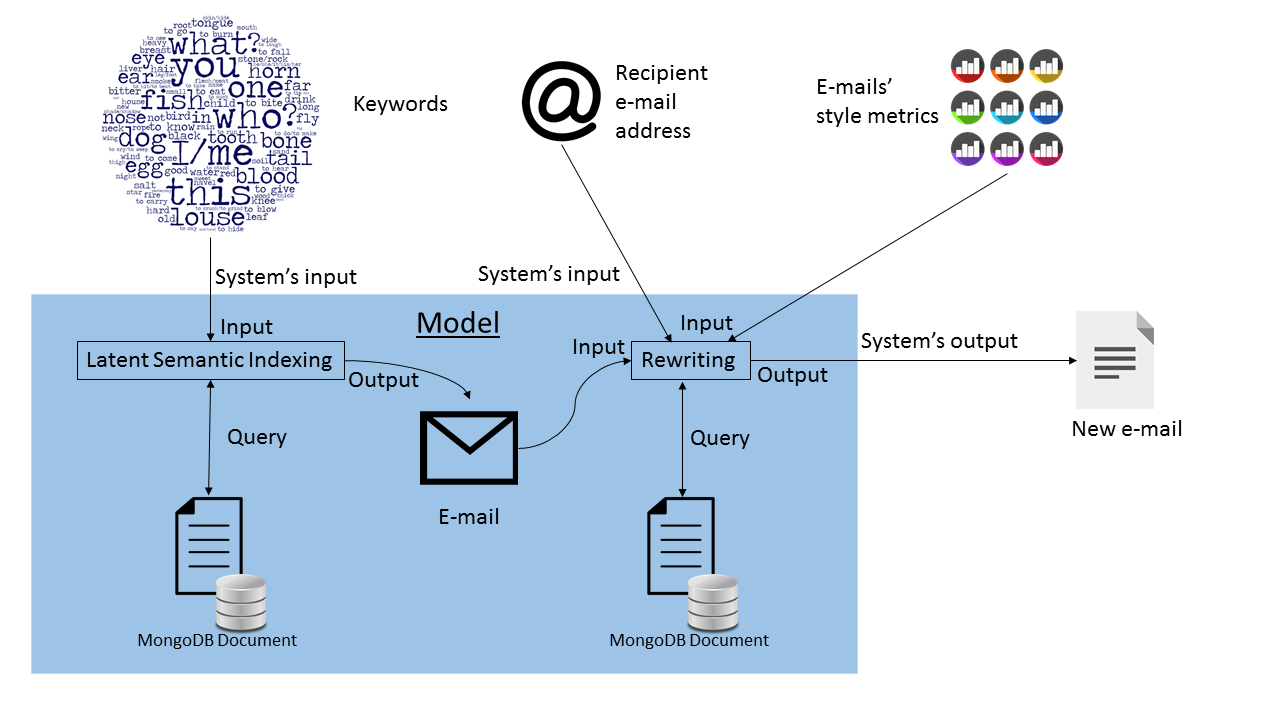
\includegraphics[width = 1.2\textwidth]{Imagenes/Bitmap/model.png}}%
	\caption{Model Architecture Diagram}%
	\label{fig:modarch}
\end{figure}

As we can see in Figure \ref{fig:modarch}, one of the required inputs of our system is the set of evaluated e-mail style metrics. Therefore it will be necessary to make use of the Analyser developed. As we have underlined, the modification of the given implementation depends on the purpose. It would be possible to remove the typographic correction phase if we want to develop a software aimed to be used by users (they will not have a good user experience if they have to correct their own e-mails before they can use the application) or if we want to take into account the typographic errors of the user with a new style marker. However, and thanks to the way the Style Analyser was implemented (with different modules as web services), any little or big modification in a module will not affect the rest of the phases. This will facilitate the reuse of the implementation developed. In this Section, we will not delve into it, instead we will just propose the model once the calculation of the different metrics is done.

Instead of trying to generate a complete e-mail, the basic idea of our model will be to rewrite one already written by the user. To achieve this, we design a model based on two phases: searching (its details are explained in Section \ref{sect:searchemail}) and rewriting (see Section \ref{sect:transemail}).

The searching phase is in charge of looking for a previously written message given a set of keywords. With this in mind, we can take advantage of the typographic corrected stored e-mails (or the preprocessed messages if this module is not used) to carry out the search. The only input that this module needs is the mentioned set of keywords, and its output is the text of the message written by the user.

The rewriting phase receives the output of the searching module. However, it will require more information in order to modify the text. For this reason, it is necessary to know who is going to be the recipient of the message and the results of the calculation of the style metrics. Once we know it, we can query the database where the classification of the different contacts is stored and, with this information, we are able to categorise the given contact. Its category will allow us to know the values of the style metrics of it and, with this information, we can choose the different methods to modify the e-mail. The output of the rewriting phase will be the new text of the message.

After having this brief introduction to the two different phases of our model, we can clearly know its inputs and outputs. At least it will be necessary to receive as input a set of keywords that describe the content of the message to be generated and its recipient. In addition we must have the style metrics previously calculated and the databases that store the texts of the messages and the established classification.

In respect of the output, it will be the generated text which is going to be the body of the e-mail sent to the given contact. Below we will detail each of the two phases that make up our system.